\documentclass{article}
\usepackage{graphicx}
\graphicspath{ {images/} }
\title{Deep Q Learning for Rocket Landing}
\date{March 2018}
\author{Ibis Prevedello}

\begin{document}
\maketitle

\section{Introduction}
The goal of this project is to study and implement a Reinforcement Learning algorithm in order to solve several games from the Gym toolkit. The algorithm used is Deep Q Learning, which uses a Deep Neural Network to learn the Q Function, also some improvements were used with Double Deep Q Learning and Prioritized Replay.

\section{Description of the problem}
Besides the idea to develop an algorithm that could be used for more than one game, this report will contain only the solution for the environment called 'Rocket Landing', which is inspired on SpaceX idea of reusable rockets.

\begin{figure}[h]
\centering
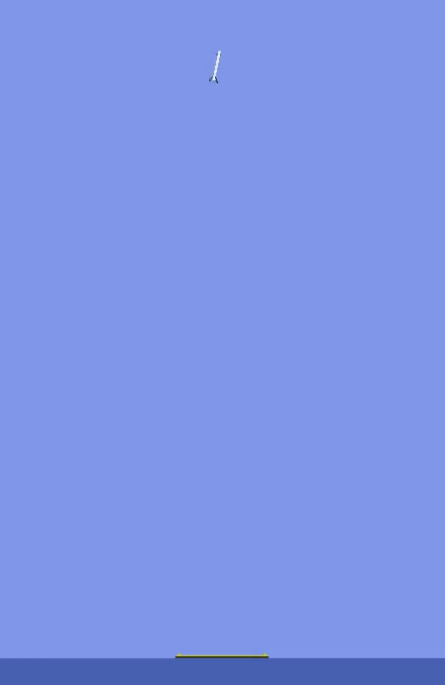
\includegraphics[scale=0.2]{environment}
\caption{Game screenshot}
\label{fig:fig1}
\end{figure}

The rocket starts from a high altitude, out of the screen, as show in \pageref{fig:fig1}, and the idea is to control it using the trusters in order to land it on a drone on the sea.

\section{Formal Model of the problem}

\section{Algorithm}
The algorithm here described is divided in tree different parts, the memory, the brain and the agent.

\section{Implementation}

\section{Results}

\section{Conclusions}

\end{document}
